% \newpage
\subsection{Управление качеством}
\label{bp:quality}
%\subsection{Управление качеством}

На предприятии выделена служба ОТК. На момент аудита контролеры по качеству дополнительно выполняют работу по подготовке оснастки для производства. Лаборатория не сертифицирована (рис. \ref{pic:6 Приборы}). Приборы проходят необходимые поверки. В лаборатории выполняются следующие анализы:

\begin{itemize}
    \item определение влажности бумаги/картона;
    \item определение влажности вырабатываемого гофрокартона; 
    \item определение сопротивления торцевому сжатию гофрокартона;
    \item определение толщины гофрокартона.
\end{itemize}

\textbf{Контроль сырья}

Контроль качества сырья при поступлении со стороны ОТК не производится. Кладовщик принимает на склад все рулоны. При выявлении замечания со стороны производства при подаче сырья на гофроагрегат составляется акт несоответствия (рис. \ref{pic:6.2 акт о браке_0001}).

\textbf{Контроль качества на гофроагрегате}

Контролеры по качеству каждую смену заполняют файл MS Excel ''Испытания на марку картона'' (рис. \ref{pic:6 рапорт отк_0001}). В файл копируется задание от специалиста по планированию. Контролер по качеству фиксирует по каждому заказу результаты измерений влажности и сопротивления торцевому сжатию. Размеры заготовки, толщину и рилевки контролирует бригада на гофроагрегате. Бригадиры сообщают контролерам по телефону или в WhatsApp о переходе на следующий заказ. Как правило образцы для анализов отбираются со второй стопы. В случае выявления несоответствий контролер сообщает бригадиру, выпуск продукции по заказу приостанавливается для внесения корректировок в технологический процесс и отладки. После запуска производится повторный отбор образцов для анализа. Выработанные некондиционные заготовки нигде не фиксируются. Бригада производит довыпуск необходимого количества заготовок на ГА (по согласованию со специалистом по планированию). Но иногда специалист по планированию узнает о перевыпуске по факту. Паллета  с некондиционной заготовкой помечается и отставляется в сторону. Бракованные заготовки  могут быть использованы на "нужды цеха" (рис. \ref{pic:7 Прокладки из брака для упаковки}) или переработаны в макулатуру (учет не ведется). При выявлении большого объема (более 500 шт или 5\% от количества по заказу ) брака ОТК составляет акт  и после разбирательства машинистов могут лишить премии.

\textbf{Контроль качества на линиях переработки}

На линиях переработки проверяется выполнение каждого заказа. После настройки оборудования бригадир вызывает контролера ОТК. Производится проверка размеров, пантонов и цвета, рилевок, просечек и т.д. Регламент производимых контролером и машинистом проверок зафиксирован в документе ДП-15 (рис. \ref{pic:6 ДП ОТК }). После устранения замечаний со стороны контролера машинист приступает к выпуску продукции по заказу. Без разрешения контролера ни один заказ не выпускается. Далее при выполнении задания постоянный контроль осуществляется бригадиром, контролер производит проверку выборочно. Бракованные изделия (рис. \ref{pic:7 Брак на линии}) и заготовки не фиксируются и используются на "нужды цеха"  или поступают в переработку в макулатуру. При выявлении большого объема (более 500 шт или 5\% от количества по заказу) брака ОТК составляет акт  и после разбирательства машинистов могут лишить премии.   
%Бланк отчета ОТК с линий производства (рис. \ref{pic:f23}) за сутки передается к руководителю службы ОТК. Данные по выпуску и браку ОТК заносят в таблицу MS Excel (рис. \ref{pic:f37}, \ref{pic:a15}). Далее все данные из отчетов ОТК распределяет по машинам, бригадам и формирует отчет  (рис. \ref{pic:a14}). Данные по расходу сырья ОТК определяет по данным отчетов по выработке из сканов отдела БППП (рис. \ref{pic:d16_1}) из колонки "расход по факту" 

%Контролер ОТК сводит итоговый отчет в сводную таблицу для вывода данных на монитор в цеху (рис. \ref{pic:a16}).

%При выявлении большого объема брака ОТК составляет акт  и после разбирательства машинистов могут лишить премии. 

%На несколько заказов приказом по предприятию (рис. \ref{pic:a18}) допускается повышенный брак из-за сложности при производстве.

%ОТК составляет сводный отчет по дням (рис. \ref{pic:a20}).

%На предприятии выделена лаборатория. 

%В лабораторию поступает задание на ГА. Лаборант берет заготовку и проводит лабораторные испытания. Лаборант измеряет показатель ЕСТ и толщину заготовки. Результаты измерений лаборант заносит на форму задания  и в журнал . 
%При значительном отклонении значений показателей от норм лаборант составляет акт и заносить показатели в журнал показателей.\
% (рис. \ref{pic:f40}).


%На перерабатывающих линиях лаборант измеряет показатель качества ЕСТ и толщину картона, проверяет геометрию и печать. Разработаны образцы недочетов, на которые можно не обращать внимание при проведении контроля качества продукции .

%По просьбе главного технолога лаборанты проводят измерение влажности на образцах сырья, поступившего на производство . Входящее сырье на склад не контролируется службой ОТК.

%Также по просьбе менеджеров лаборанты определяют состав образцов от клиента и марку.
% \clearpage
%При поступлении заготовки в цех контролер ОТК проверяет заготовки на механические повреждения и при выявлении брака составляет акт и делает фото (рис. \ref{pic:a64}). Претензии к поставщику контролер ОТК выставляет при превышении количества брака более чем на 2 процента от общего объема поставки.

%Далее контролер ОТК начинает претензионную работу: отправляет претензию и ожидает ответа от поставщика. После прихода письма от поставщика 
% (рис. \ref{pic:a59}) 
%и при появлении представителей поставщика контролер ОТК собирает комиссию и составляет акт отбраковки (рис. \ref{pic:a60}). 

%Если продукция подлежит возврату, контролер ОТК составляет акт выбраковки и сопроводительные документы (рис. \ref{pic:a61}, рис. \ref{pic:a62}).

%Претензии от покупателей по готовой продукции поступают менеджерам.
%При появлении претензии от покупателя на ГП менеджеры стараются решить на месте. Документы по претензиям от потребителей не ведутся. 

%На линии контролер ОТК проверяет размеры, качество печати и толщину картона толщиномером.
%Контролер ОТК ведет журнал измерения толщины по номенклатуре выпускаемых изделий (рис. \ref{pic:a63}).
\begin{figure}
\begin{center}
  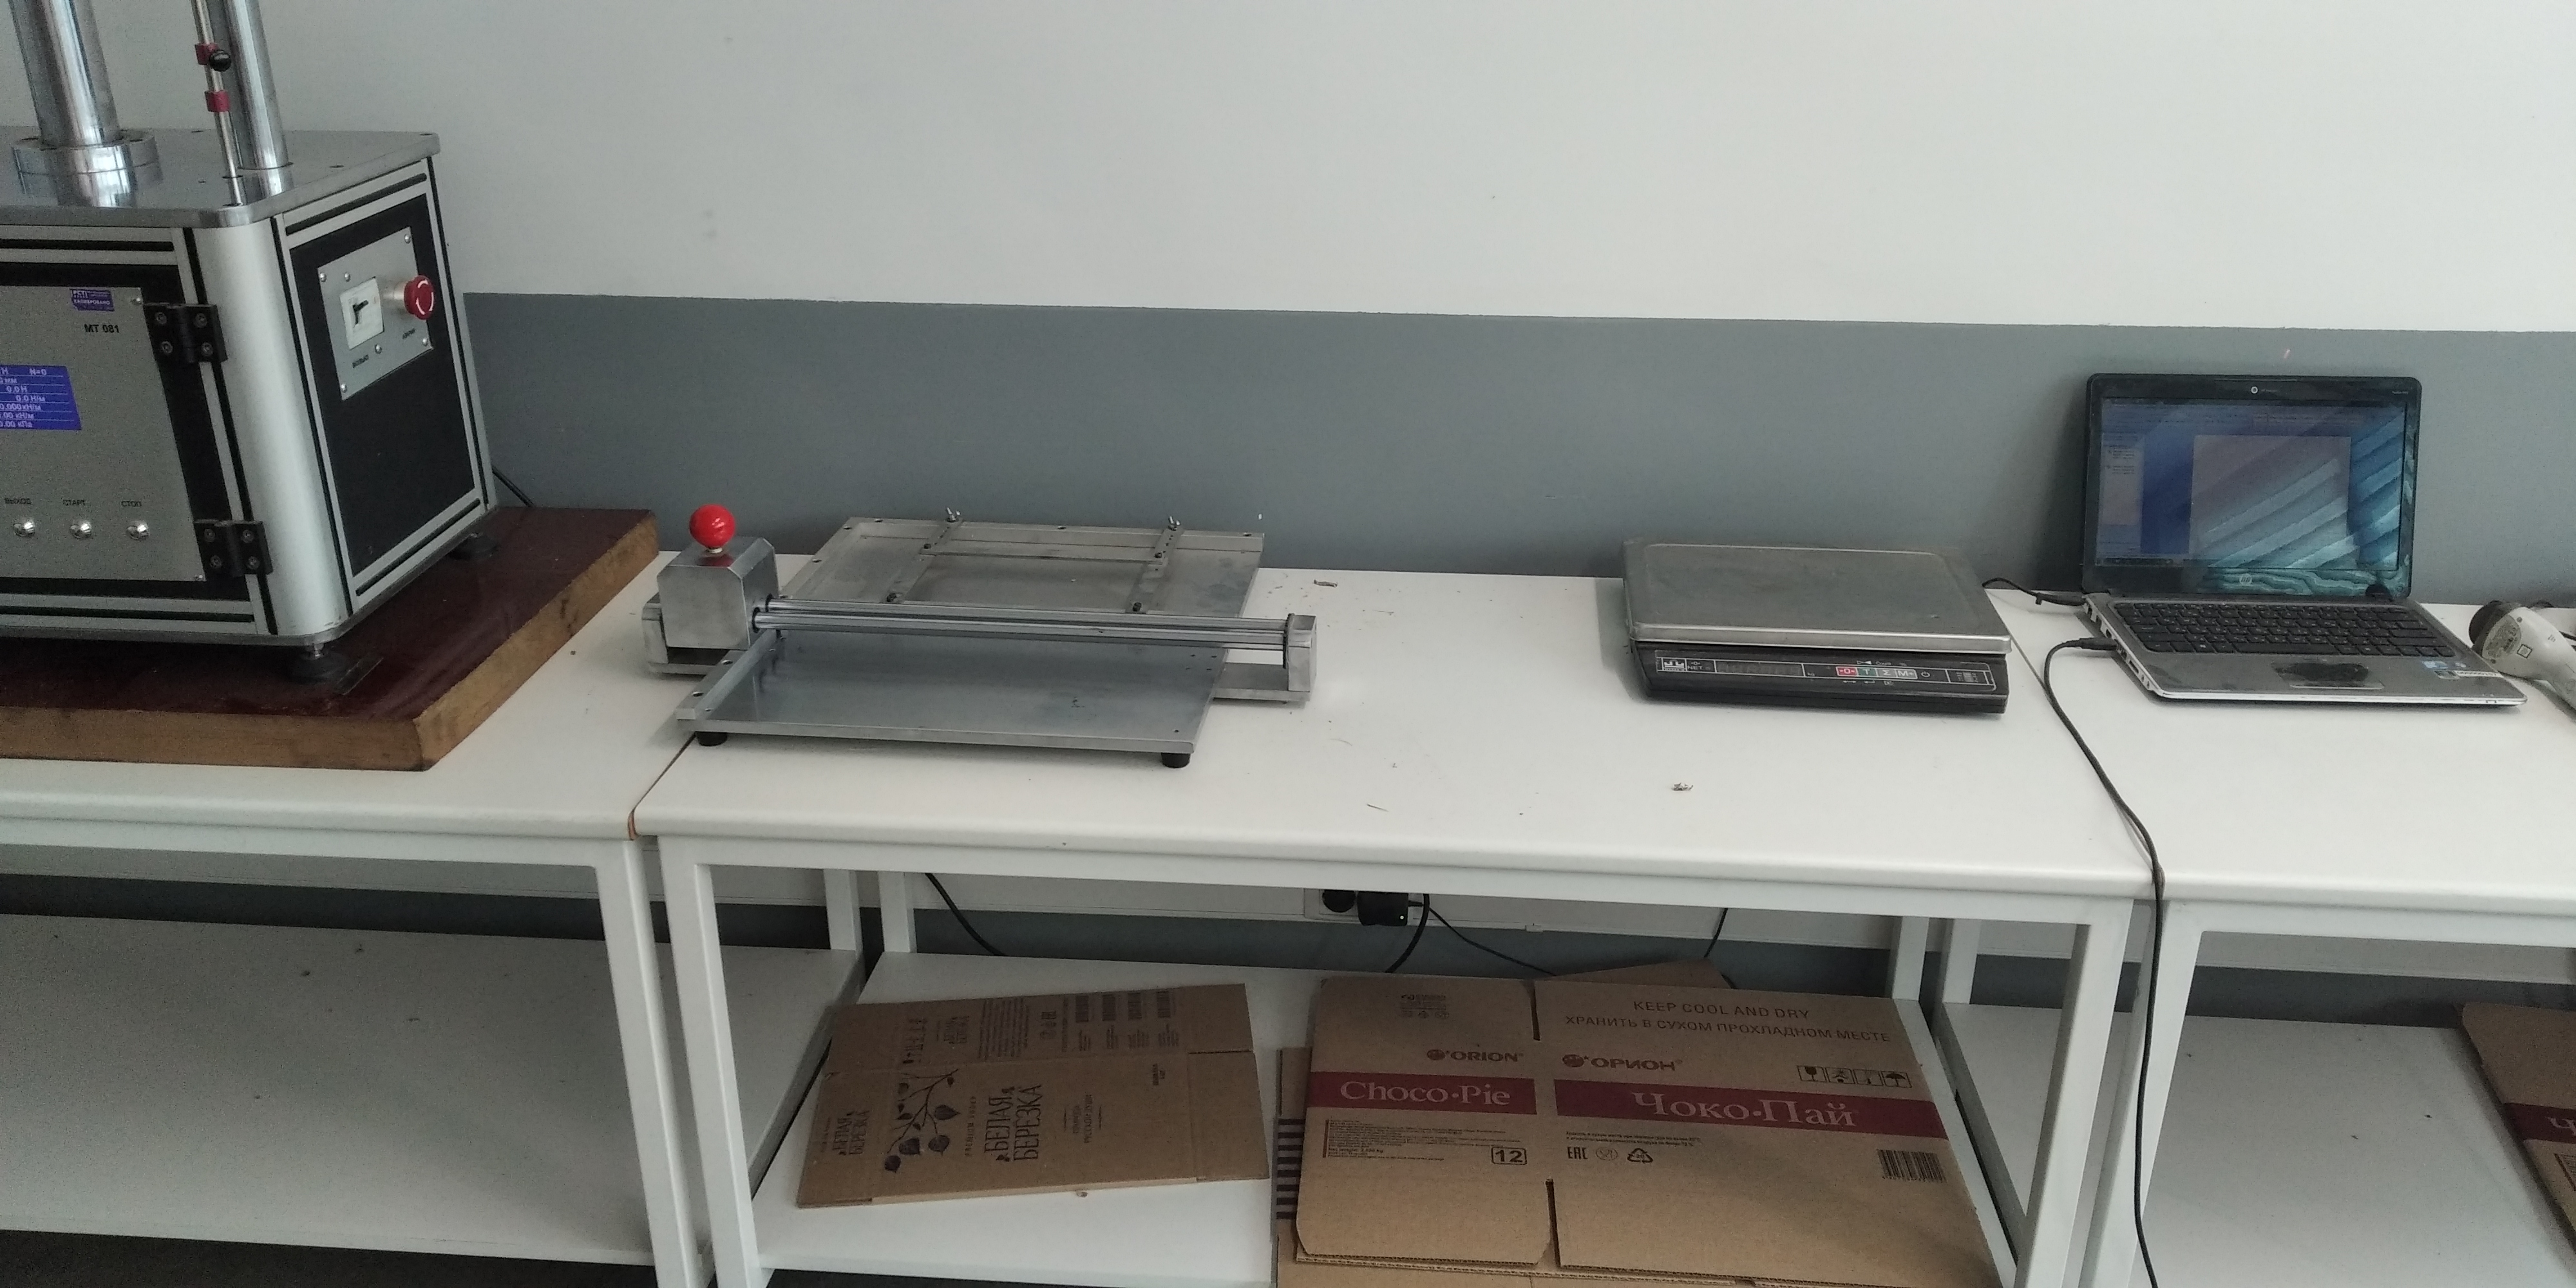
\includegraphics[height=0.94\textheight, width=0.94\textwidth, keepaspectratio]{Pics 1/6 Приборы.jpg}
\end{center}
  \caption{Лаборатория}
  \label{pic:6 Приборы}
\end{figure}

\begin{figure}
\begin{center}
  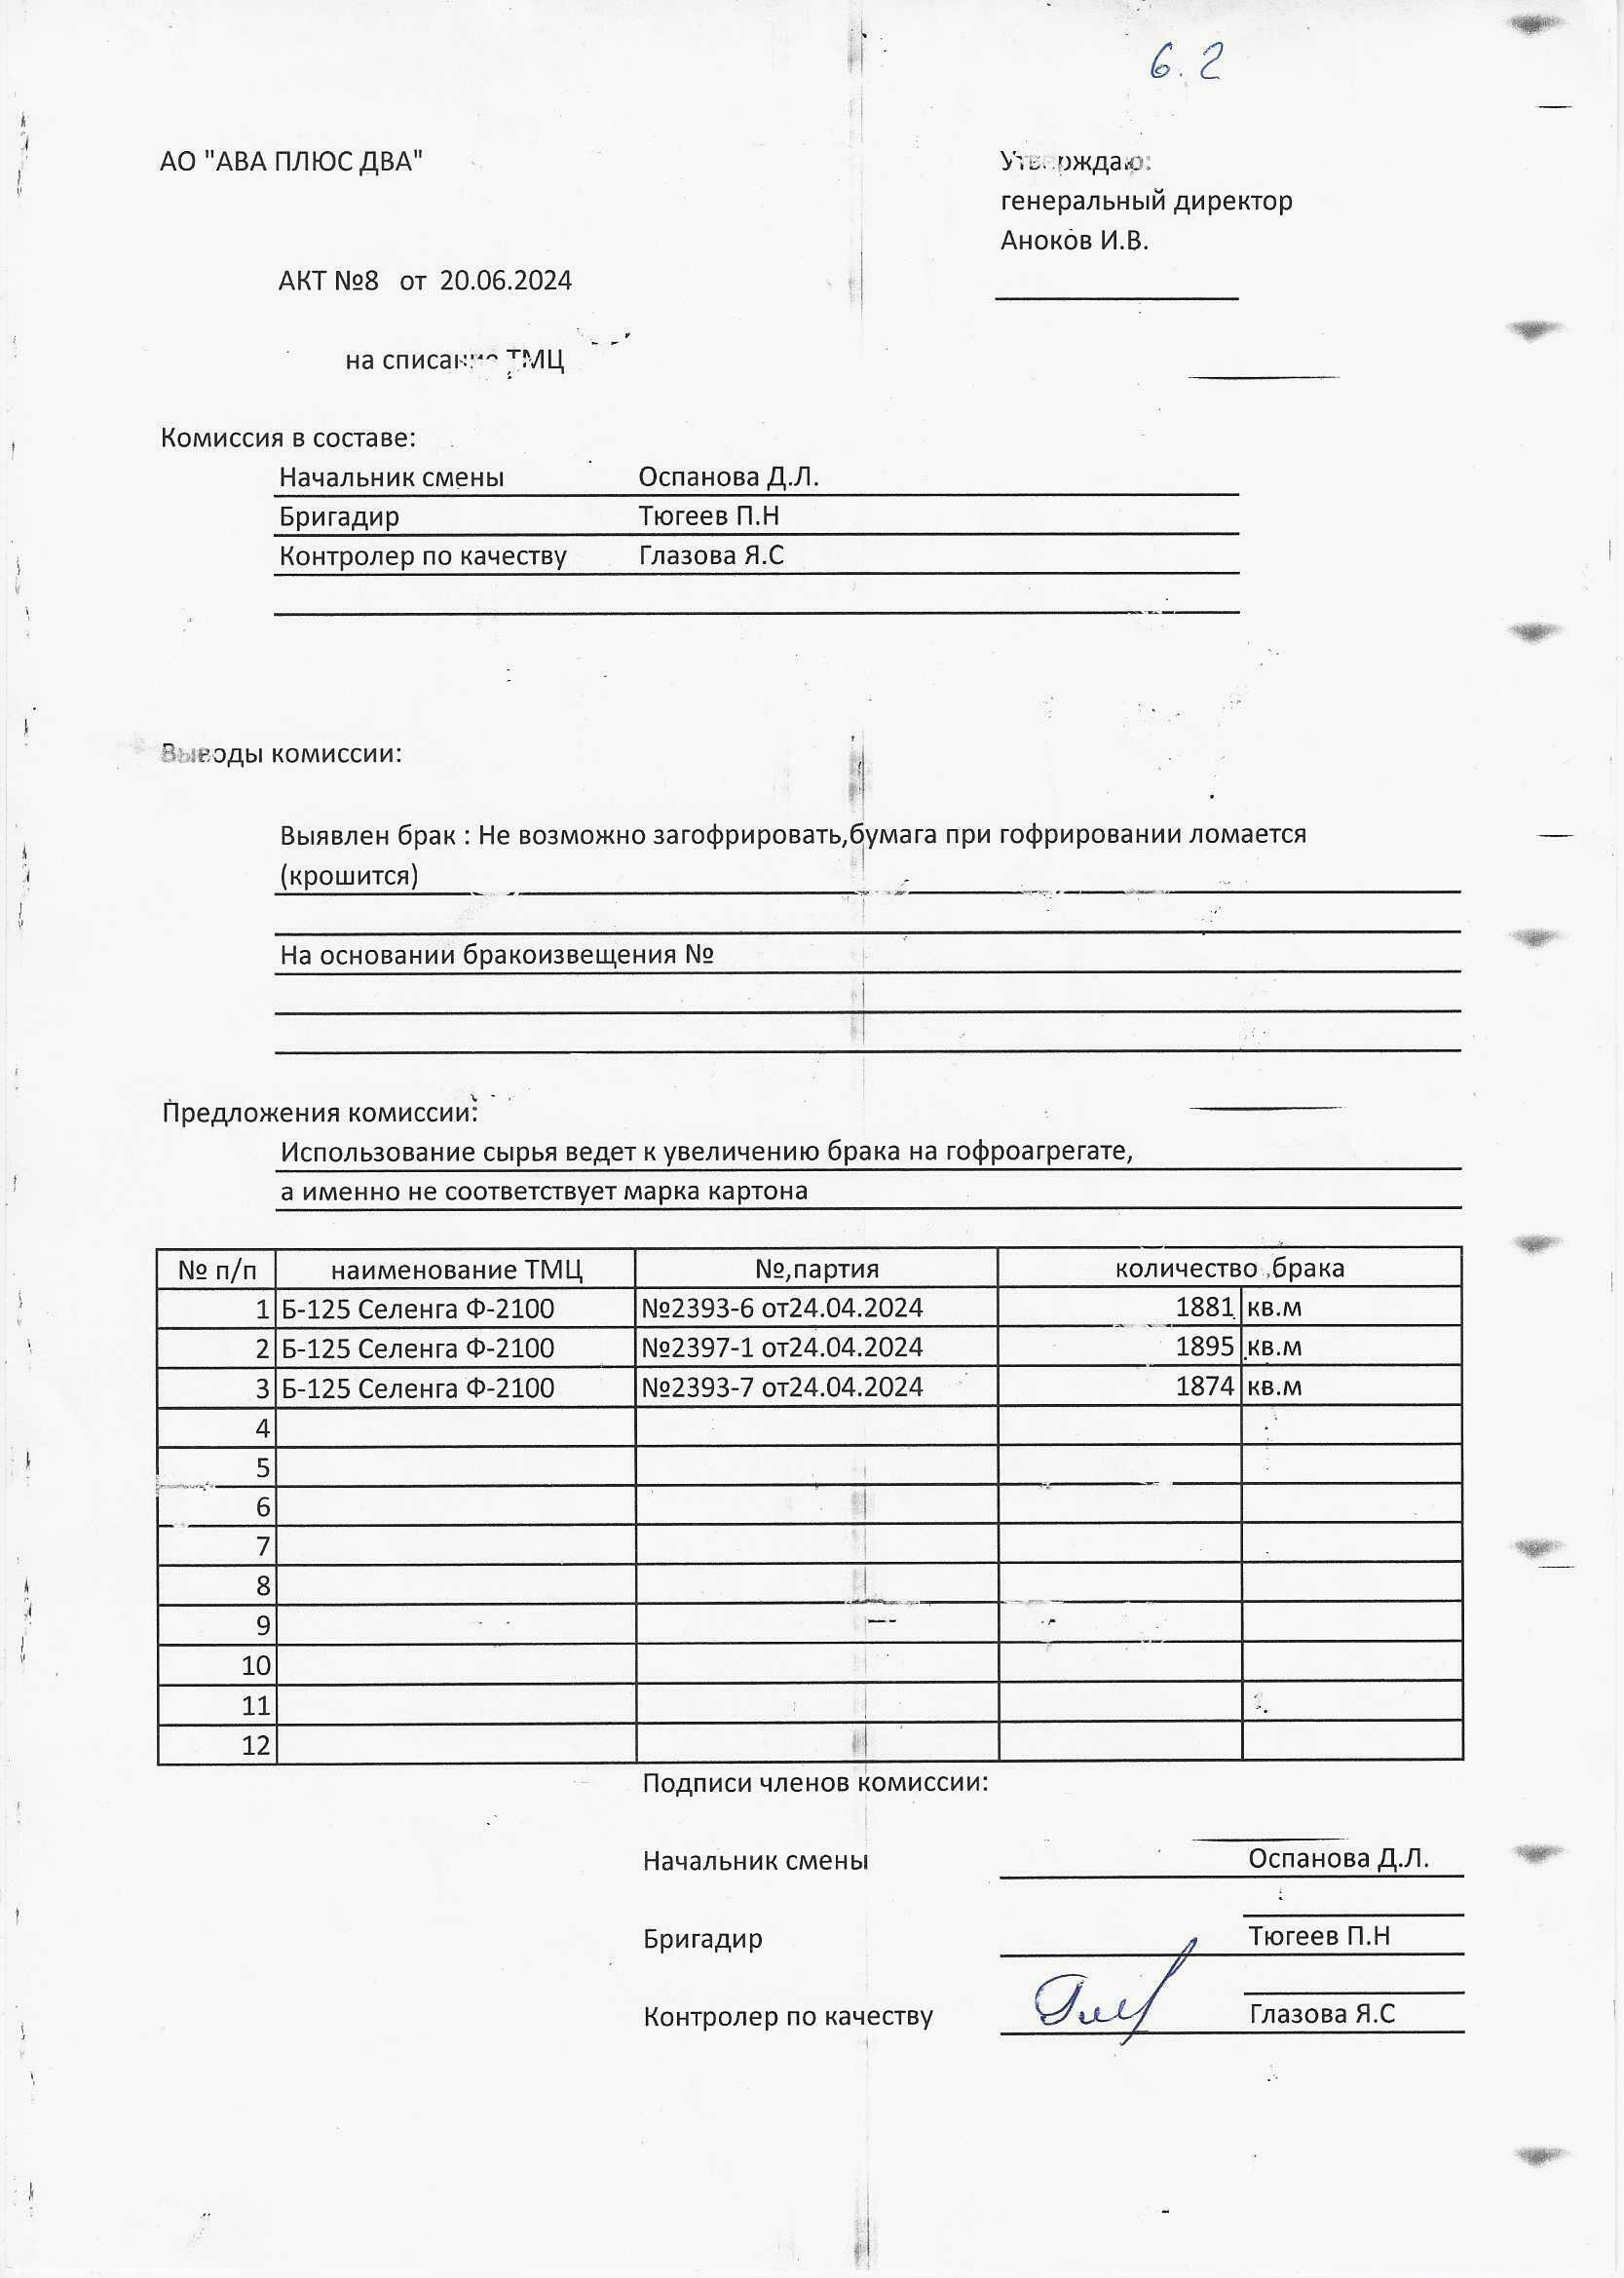
\includegraphics[height=0.94\textheight, width=0.94\textwidth, keepaspectratio]{Pics 1/6.2 акт о браке_0001.jpg}
\end{center}
  \caption{Пример акта о браке}
  \label{pic:6.2 акт о браке_0001}
\end{figure}

\begin{figure}
\begin{center}
  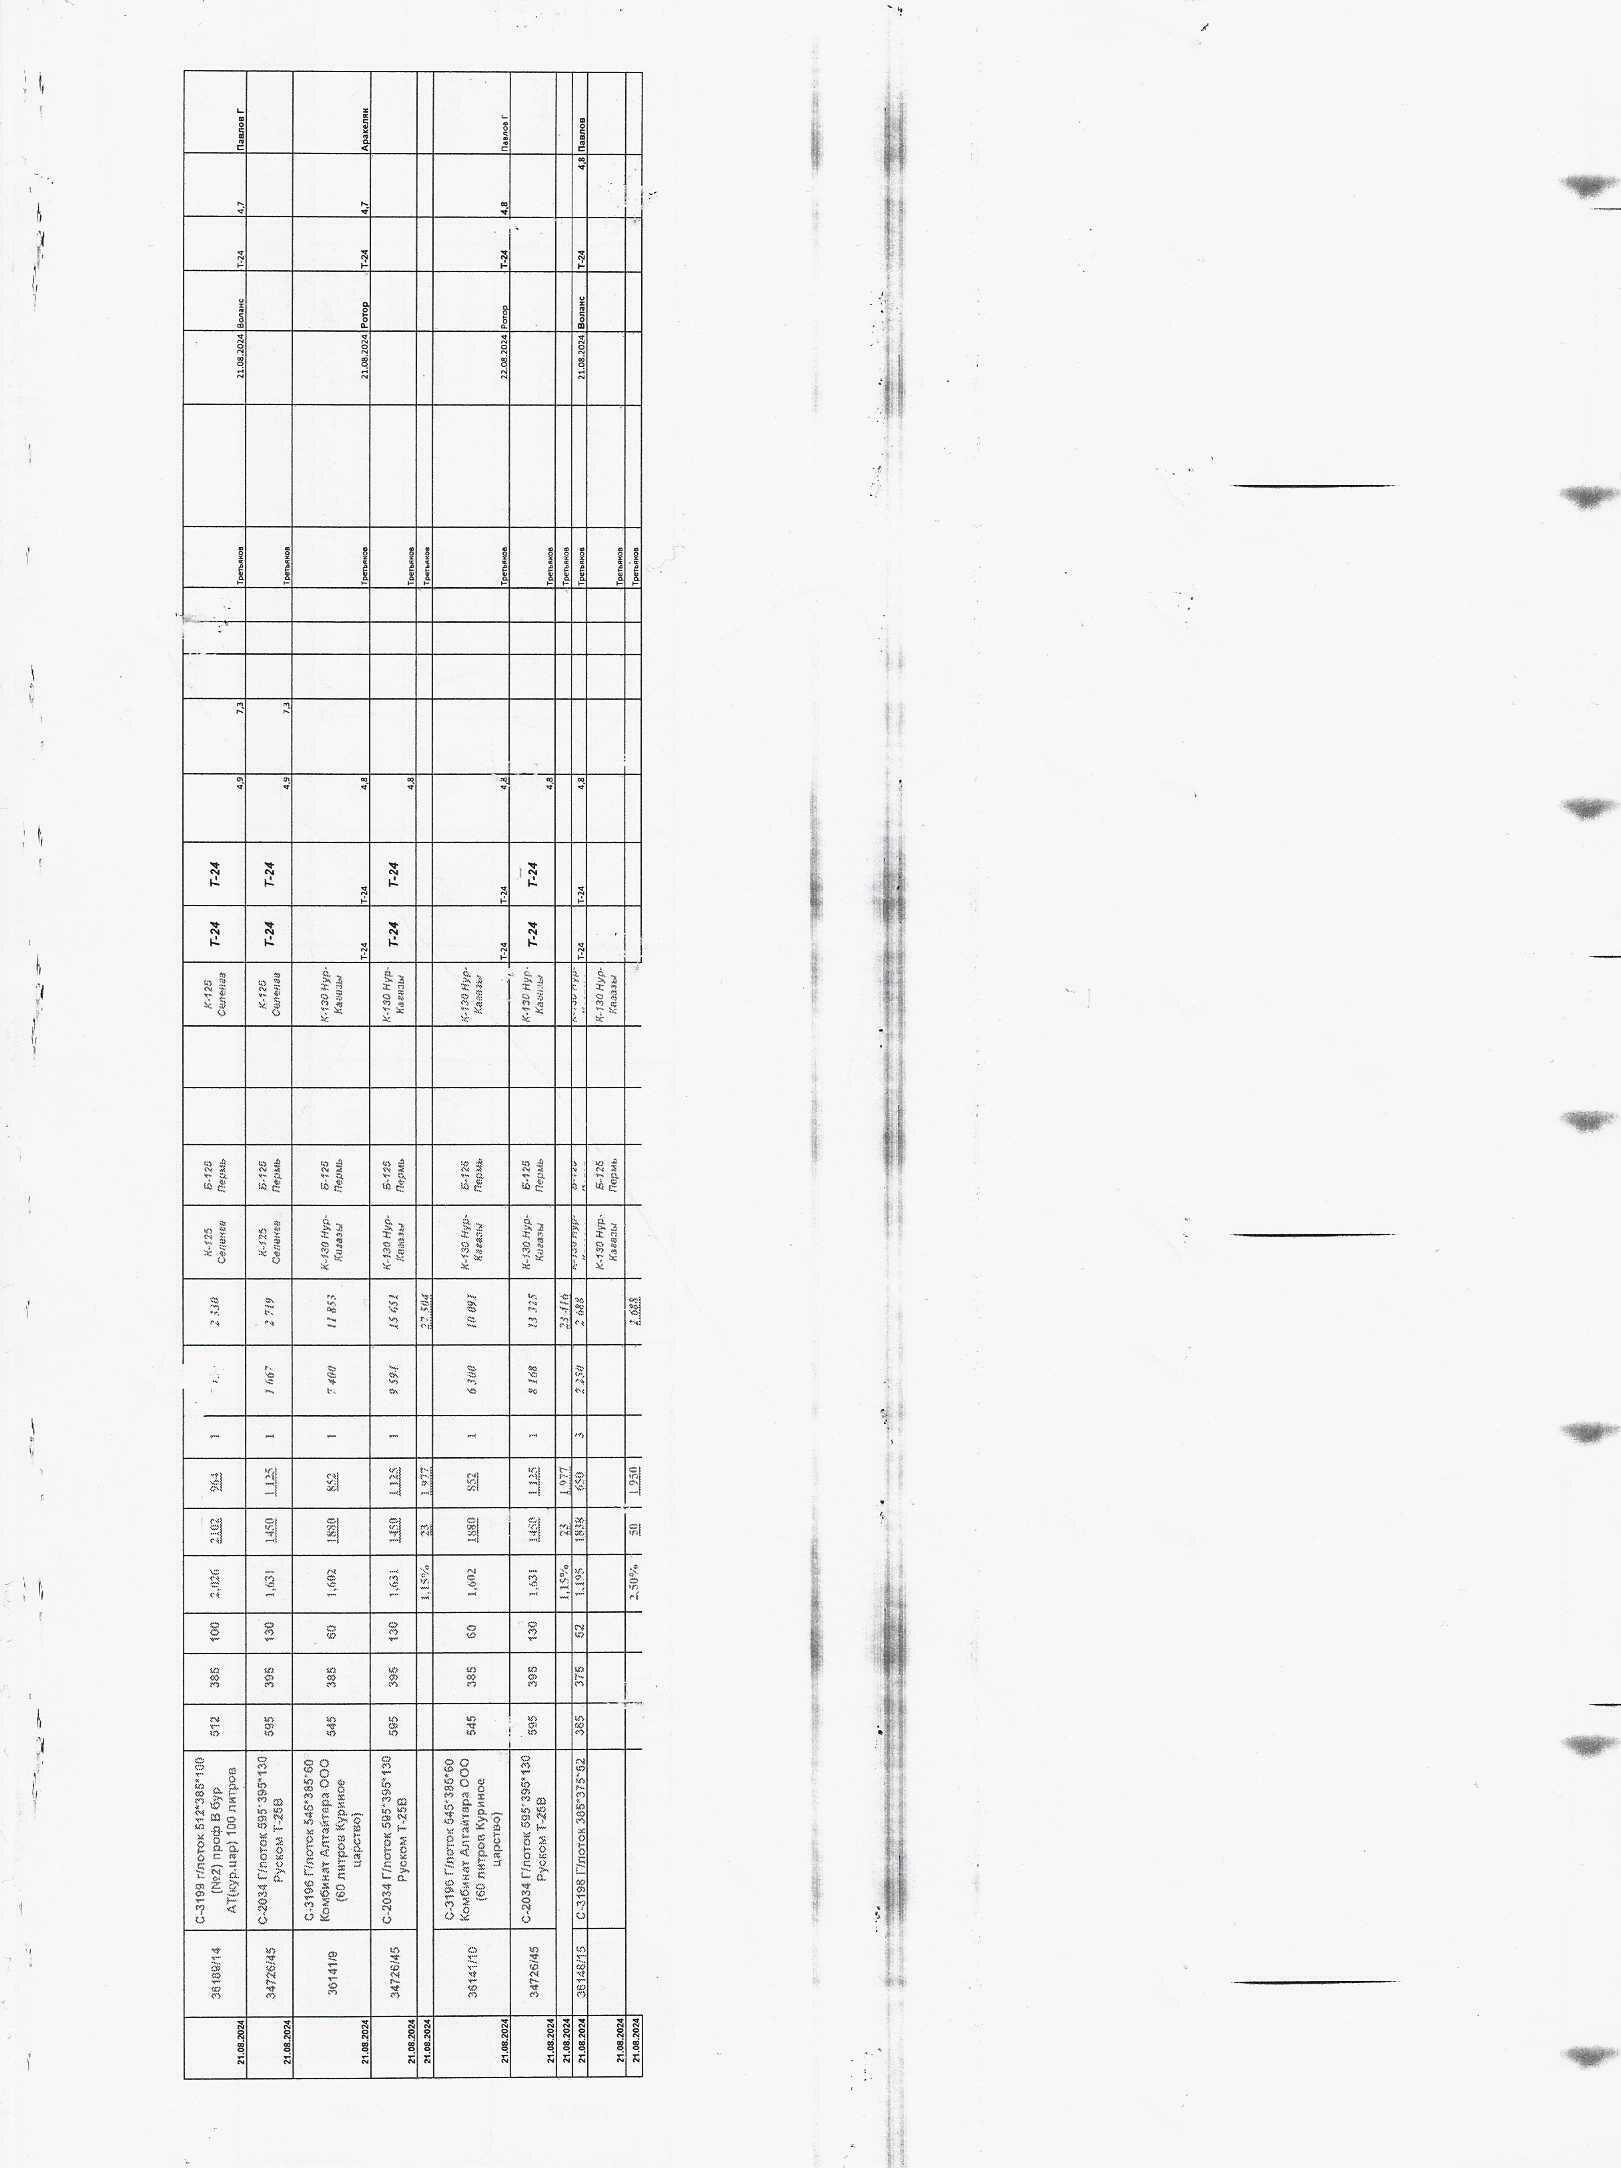
\includegraphics[height=0.94\textheight, width=0.94\textwidth, keepaspectratio]{Pics 1/6 рапорт отк_0001.jpg}
\end{center}
  \caption{Рапорт ОТК}
  \label{pic:6 рапорт отк_0001}
\end{figure}

\begin{figure}
\begin{center}
  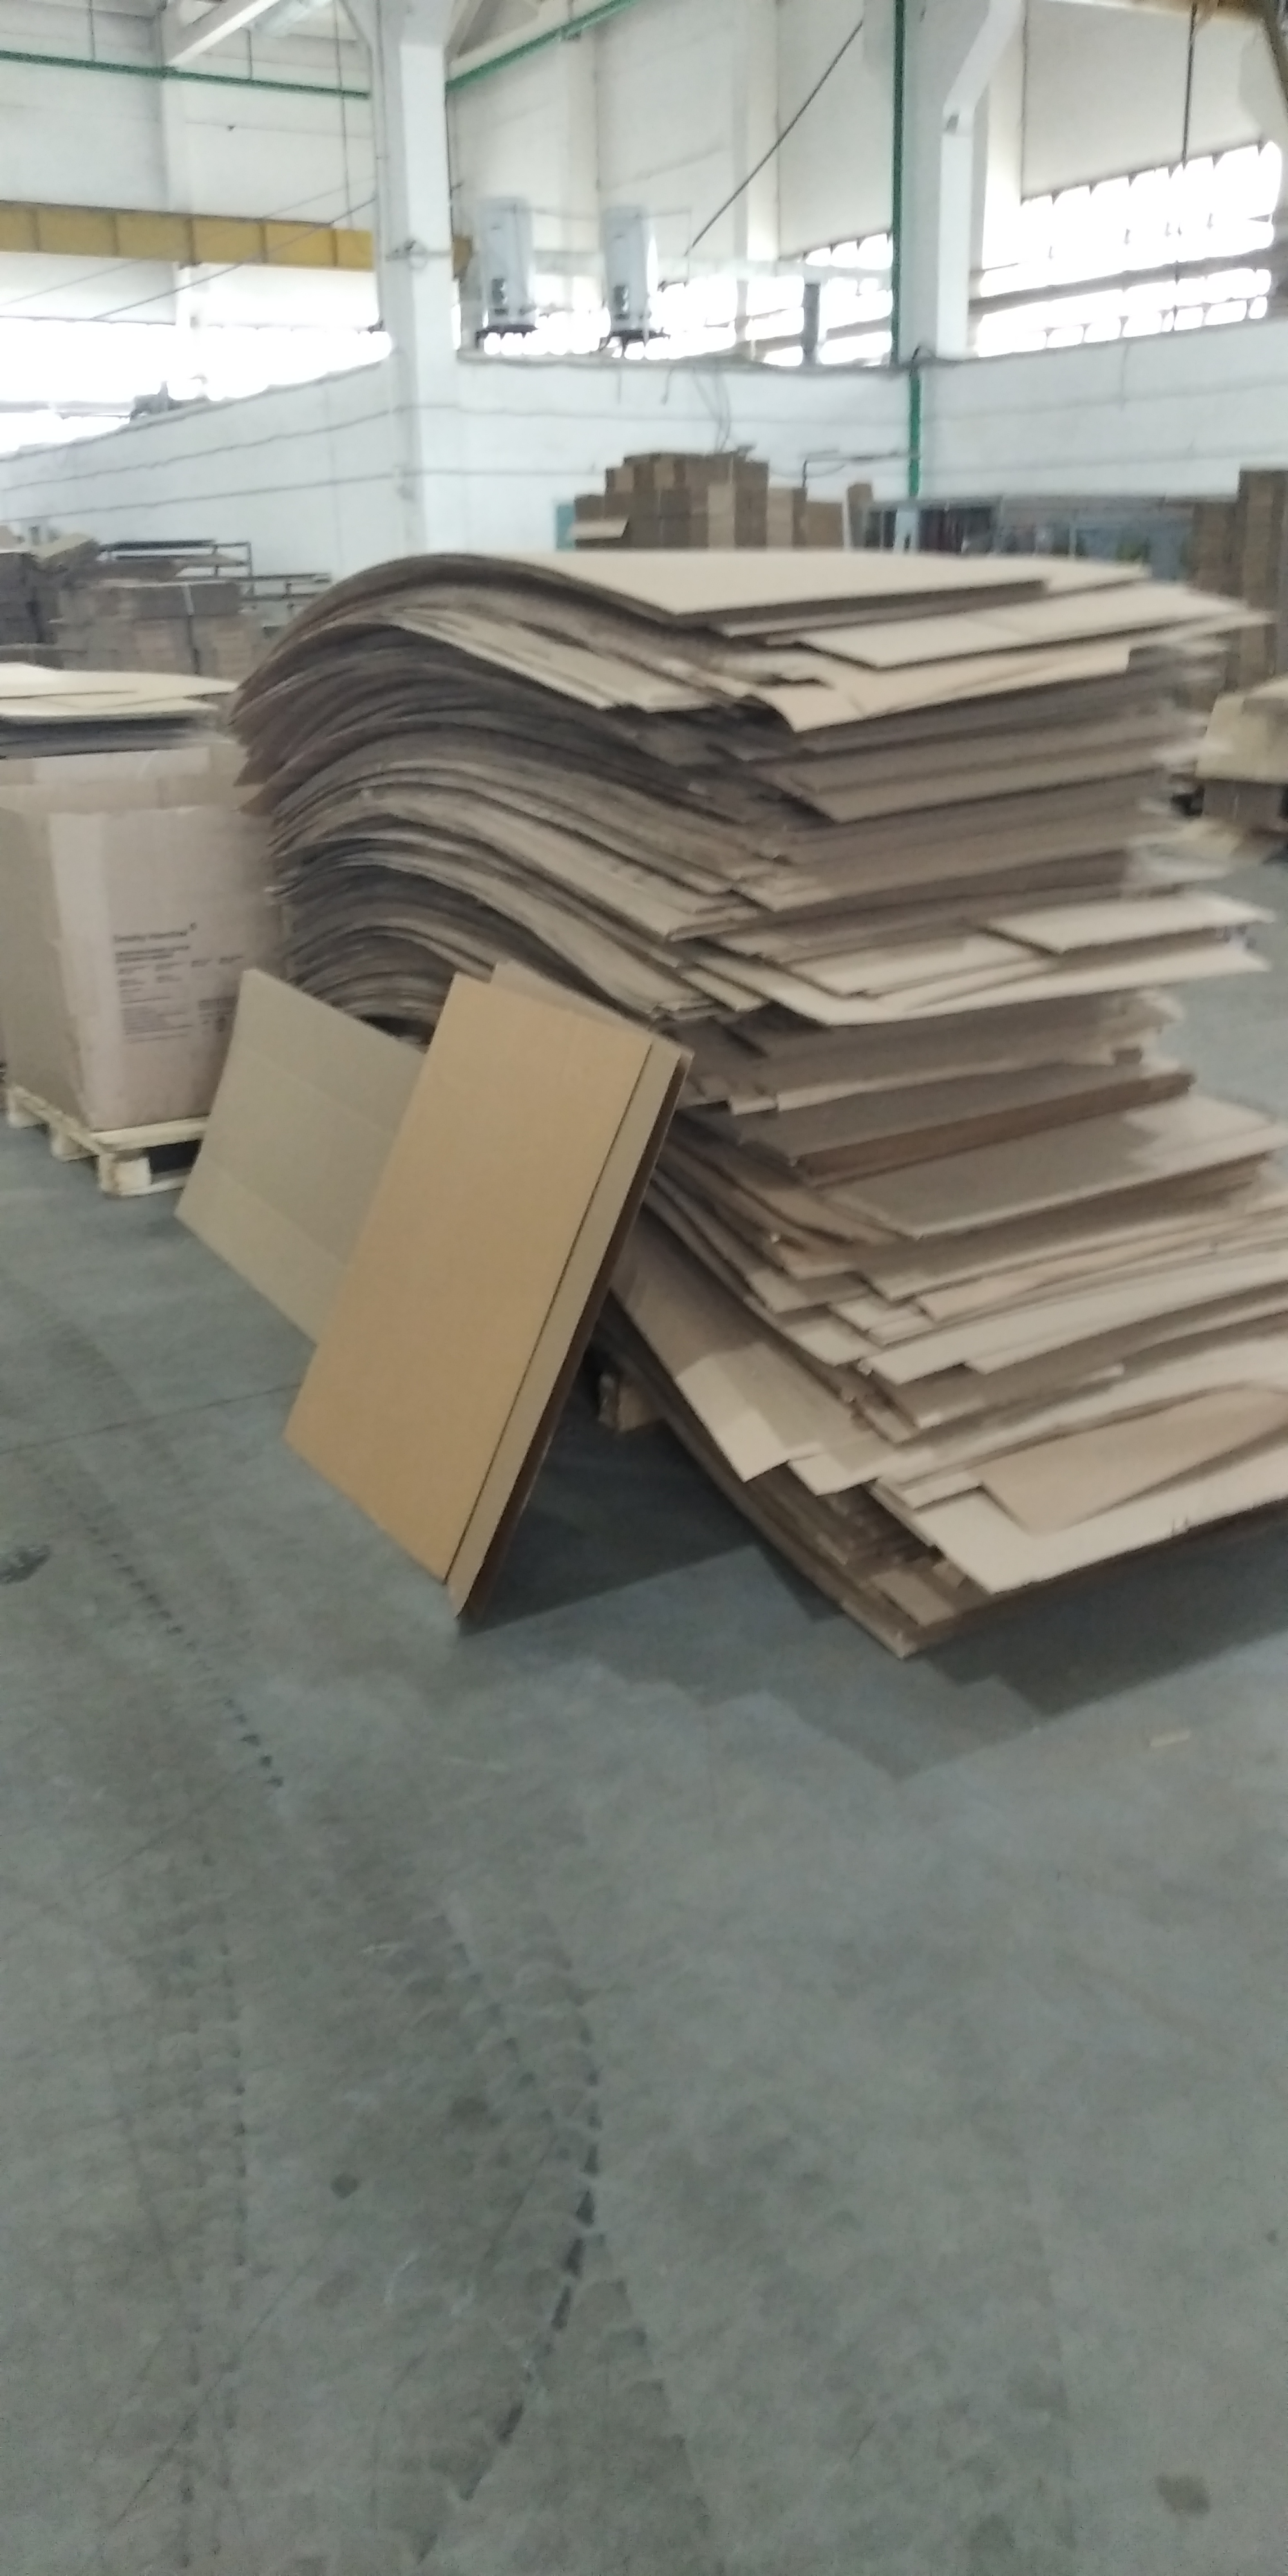
\includegraphics[height=0.94\textheight, width=0.94\textwidth, keepaspectratio]{Pics 1/7 Прокладки из брака для упаковки.jpg }
\end{center}
  \caption{Некондиционные заготовки}
  \label{pic:7 Прокладки из брака для упаковки}
\end{figure}

\begin{figure}
\begin{center}
  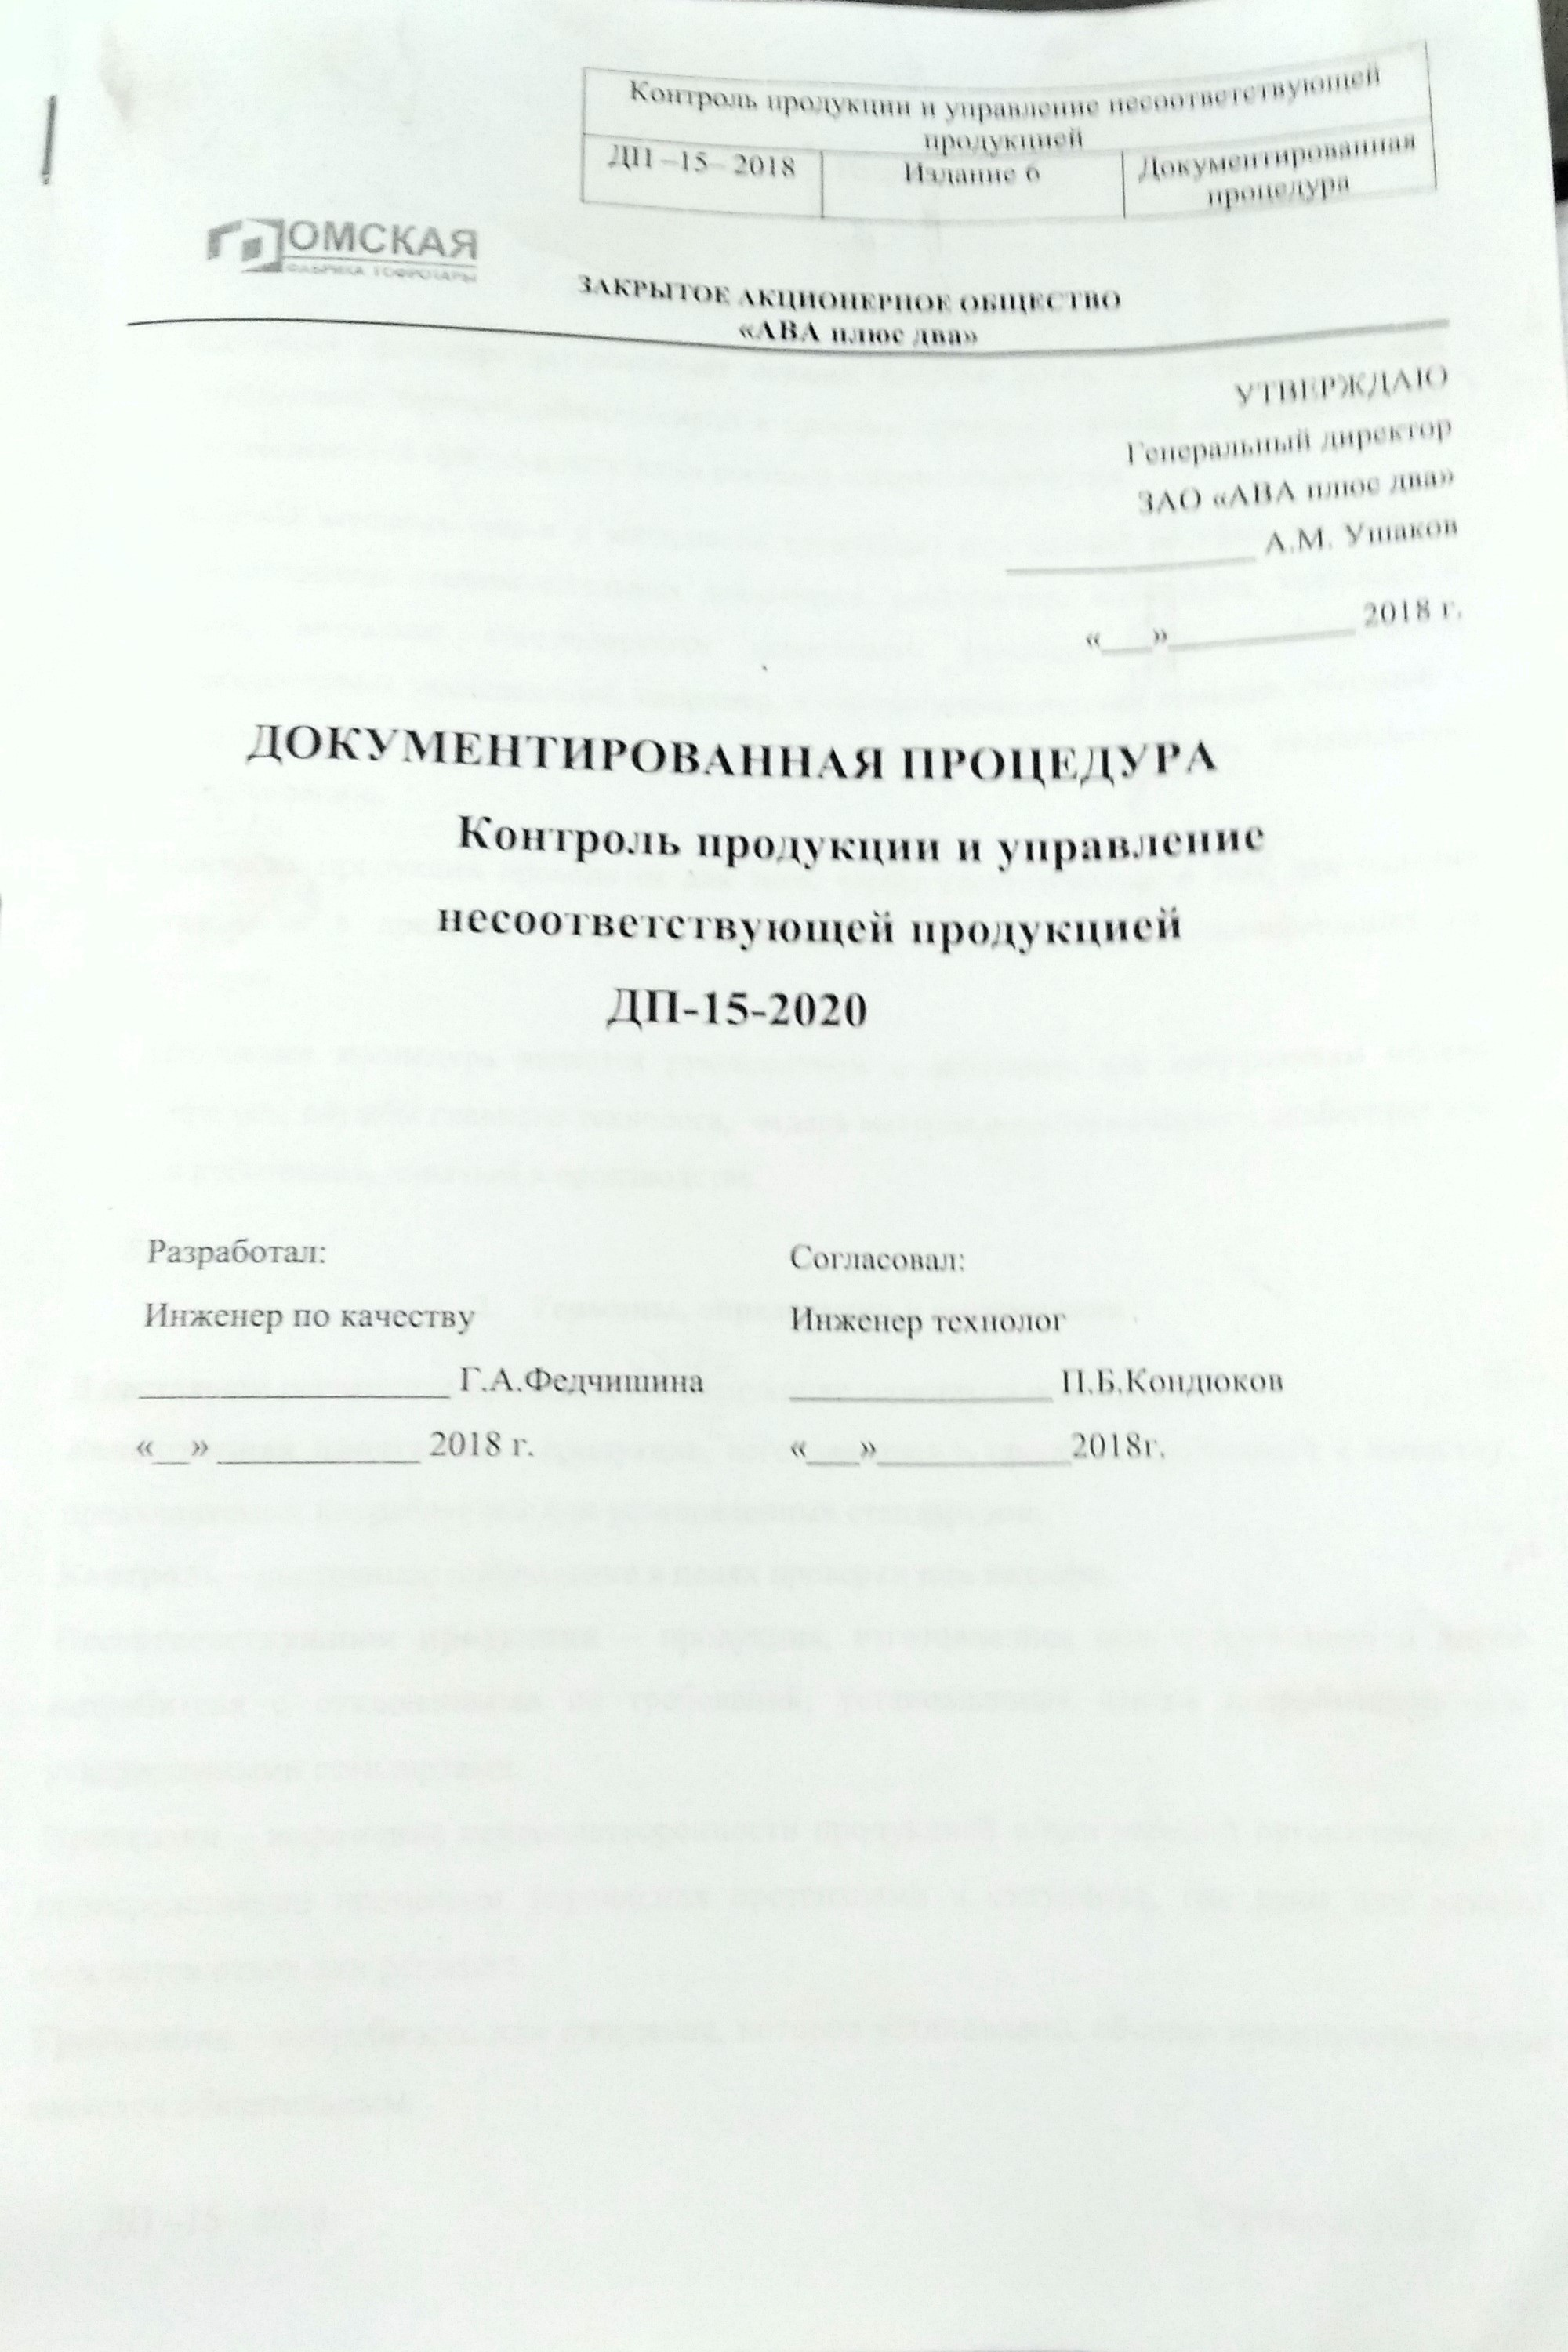
\includegraphics[height=0.94\textheight, width=0.94\textwidth, keepaspectratio]{Pics 1/6 ДП ОТК.jpg }
\end{center}
  \caption{Документ ДП-15}
  \label{pic:6 ДП ОТК }
\end{figure}

\begin{figure}
\begin{center}
  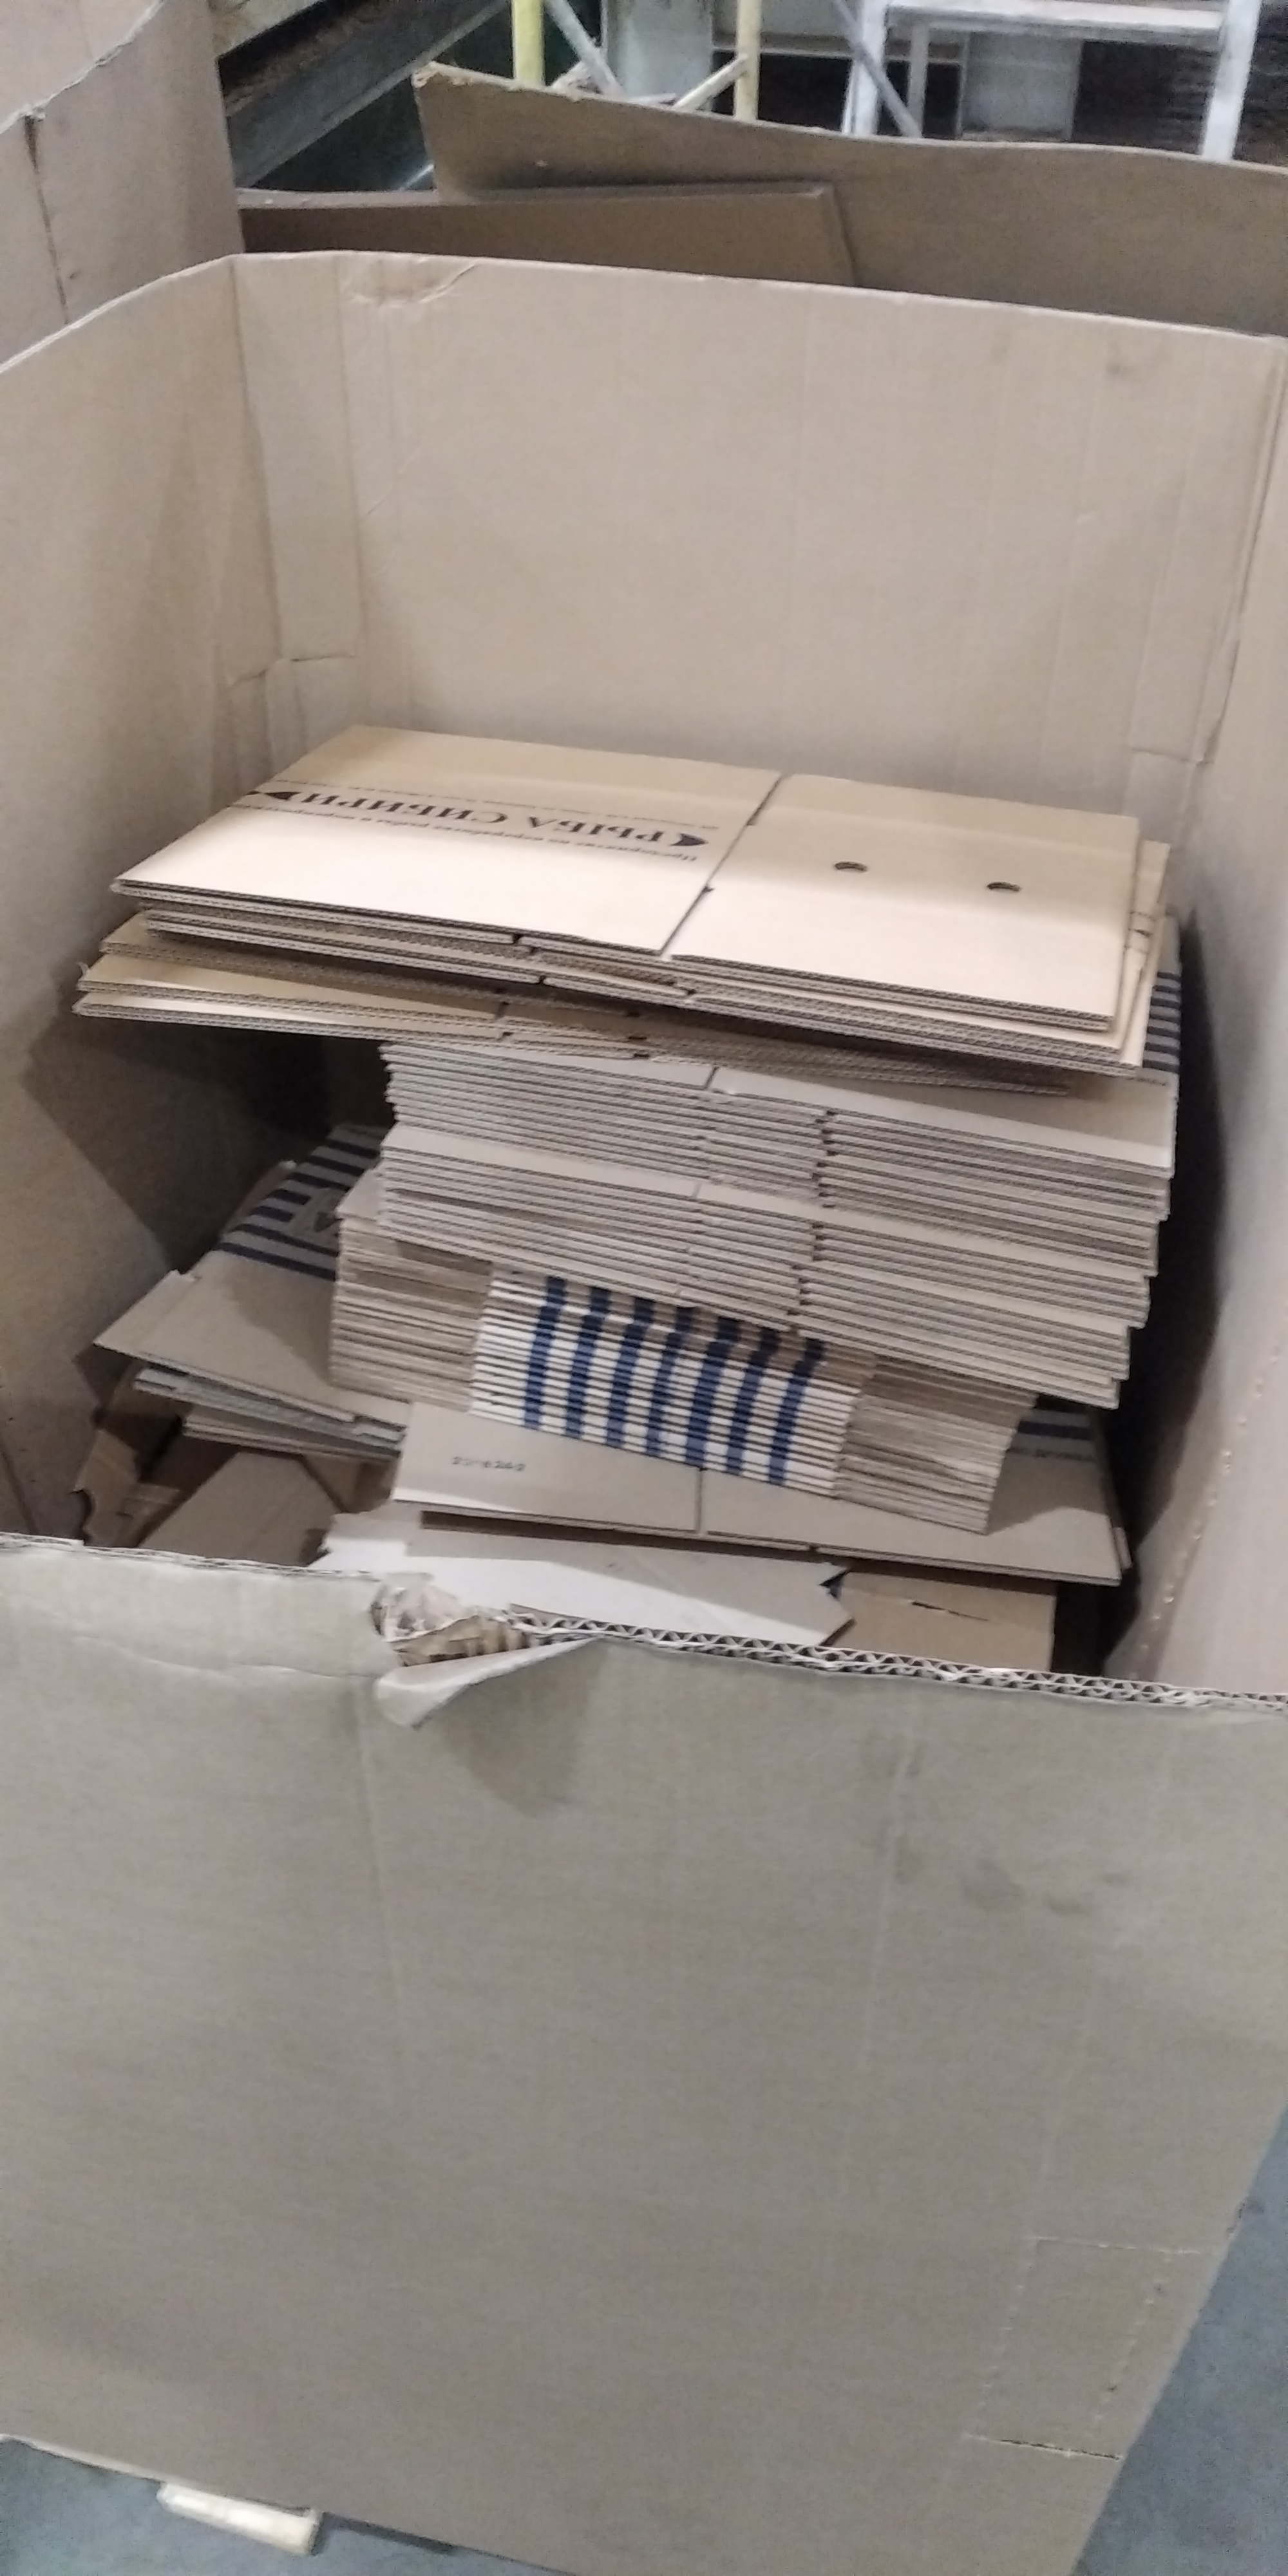
\includegraphics[height=0.94\textheight, width=0.94\textwidth, keepaspectratio]{Pics 1/7 Брак на линии.jpg }
\end{center}
  \caption{Бракованные изделия на линии переработки}
  \label{pic:7 Брак на линии}
\end{figure}

\clearpage
\ifx \notincludehead\undefined
\normalsize
\end{document}
\fi